\documentclass[class=article, crop=false]{standalone}
\usepackage[subpreambles=true]{standalone}
\usepackage{import}
\usepackage{amsmath}
\usepackage{enumitem} % Format list spacing 

\begin{document}
\begingroup
\setlength{\parskip}{0.85em}

%%%%%%%%%%%%%%%%%%%%%%%%%%%%%%%%%%%% Gauge Implementations %%%%%%%%%%%%%%%%%%%%%%%%%%%%%%%%%%%%

\subsection{Gauge Implementations}

The following \term{Gauge Implementation} is used throughout this whitepaper.

%%%%%%%%%%%%%%%%%%%%%% Cultivation Factor %%%%%%%%%%%%%%%%%%%%%%

\subsubsection{Cultivation Factor Gauge}\label{sec:cultivation-factor}

The protocol increases the \term{Cultivation Factor} when Pinto is \term{Sown} in all \term{Soil} in the previous \term{Season}. Conversely, if Pinto is not \term{Sown} in all \term{Soil} in the previous \term{Season}, the protocol decreases the \term{Cultivation Factor} or leaves it unchanged.

$\mathfrak{C}_{t}$ was initialized to $0.5$ at the time of PI-6\fref{pinto.money/pi-6} deployment (\textit{i.e.}, $t$ = $2710$).

The \term{Cultivation Factor} during $t$ is based on (1) the \term{Cultivation Factor} during the previous \term{Season}, (2) the change in \term{Cultivation Factor} this \term{Season} ($\Delta \mathfrak{C}_{t}$), such that $\Delta \mathfrak{C}_{t} \in \{j \times 10^{-8} \mid j \in \mathbb{Z}^{+} \}$, (3) the time weighted average price of \Pinto1 over the previous \term{Season}, capped at $1$, in the \term{Well} whose non-Pinto USD-denominated liquidity, weighted by $f^{\mathscr{W}^{\lambda}}$, is greatest ($P_{\overline{t-1}}^{\mathfrak{C}}$), such that $P_{\overline{t-1}}^{\mathfrak{C}} \in \{j \times 10^{-6} \mid j \in \mathbb{N} \}$, (4) whether Pinto were \term{Sown} in all or most \term{Soil} in the previous \term{Season}, (5) changing demand for \term{Soil}, (6) $H_{t-1}$, and (7) the \term{Cultivation Temperature} during $t$.

\begin{keepunit}
We define $\Delta \mathfrak{C}_{t}$ for a given $R_{t-1}^{D}$, $R^{D^{\text{upper}}}$ and $R^{D^{\text{lower}}}$ as:

    $$
        \Delta \mathfrak{C}_{t} =
            0.02 - \frac{\text{max(min($R_{t-1}^{D}$, $R^{D^{\text{upper}}}$)} - \text{$R^{D^{\text{lower}}}$}, 0)} {\text{$R^{D^{\text{upper}}}$} - \text{$R^{D^{\text{lower}}}$}} \times 0.015
    $$
\end{keepunit}

\begin{keepunit}
We define the maximum amount of \term{Soil} remaining for Pinto to be considered \term{Sown} in most \term{Soil} in \term{Season} $t$, measured at the \term{Maximum Temperature} ($S_t^{\text{most}}$), such that $S_t^{\text{most}} \in \{j \times 10^{-6} \mid j \in \mathbb{N} \}$, as:\looseness=-1

    $$
        S_t^{\text{most}} = S_t^{\text{all}} + \frac{S_t^{\text{start}}-S_t^{\text{all}}}{5}
    $$
\end{keepunit}

\begin{keepunit}
The protocol considers most \term{Soil} sold after the first \term{Sow} in \term{Season} $t$ that leaves at least $S_t^{\text{all}}$ and at most $S_t^{\text{most}}$ \term{Soil} remaining, measured at the \term{Maximum Temperature}.

\begin{figure}[H]
    \centering
    \documentclass{standalone}
\usepackage{tikz,pgf,amssymb,bm}

\begin{document}

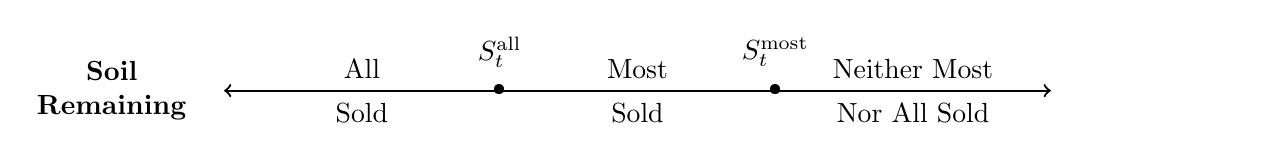
\begin{tikzpicture}[scale=7]

\node [draw=none] at (1,0.04) {Neither Most};
\node [draw=none] at (1,-0.04) {Nor All Sold};

\node [draw=none] at (0.5,0.04) {Most};
\node [draw=none] at (0.5,-0.04) {Sold};

\node [draw=none] at (0,0.04) {All};
\node [draw=none] at (0,-0.04) {Sold};

\node [draw=none] at (0.25,0.07) {$S_t^{\text{all}}$};
\node [draw=none] at (0.75,0.07) {$S_t^{\text{most}}$};

\foreach \Point in {0.25, 0.75}{
    \node[label={[label distance=1mm]:\rotatebox{0}{}}] at (\Point,0) {\textbullet};
}
\draw[thick,<->,color=black] (-0.25,0) -- (1.25,0); % Draw line
\node [draw=none, anchor=east, align=center] at (-0.30,0) {\textbf{Soil}\\\textbf{Remaining}}; % Chart label
\node [draw=none, anchor=west, align=center, text=white] at (1.30,0) {\textbf{Soil}\\\textbf{Remaining}}; % Added to center chart

\end{tikzpicture}

\end{document}

    \vspace*{-7mm}
    \caption{Soil Sold}
    \label{Soil Sold}
\end{figure}
\end{keepunit}

The \term{Cultivation Temperature} ($H_t^{\mathfrak{C}}$), such that $H_t^{\mathfrak{C}} \in \{j \times 10^{-6} \mid j \in \mathbb{N} \}$, is the \term{Maximum Temperature} in the last \term{Season} in which Pinto were \term{Sown} in all or most \term{Soil} and demand for \term{Soil} was steady or increasing. It was initialized to $0$ at the time of PI-10\fref{pinto.money/pi-10} deployment.

\begin{keepunit}
We define $H_t^{\mathfrak{C}}$ for a given $H_{t-1}$, the amount of \term{Soil} sold, changing demand for \term{Soil} and $H_{t-1}^{\mathfrak{C}}$ as:

    $$
        H_t^{\mathfrak{C}} =
        \begin{cases}
            H_{t-1} & \begin{gathered}\text{if Pinto were Sown in all or most Soil in }t-1\\\mkern6mu \&\& \mkern6mu\text{demand is not decreasing}\end{gathered}\\
            H_{t-1}^{\mathfrak{C}} & \text{else}
        \end{cases}
    $$
\end{keepunit}

\begin{keepunit}
Therefore, we define $\mathfrak{C}_{t}$ as:

    $$
        \mathfrak{C}_{t} =
        \begin{cases}
            \min(1,\ \mathfrak{C}_{t-1}+\Delta\mathfrak{C}_{t}\times P_{\overline{t-1}}^{\mathfrak{C}})
                & \text{if Pinto were Sown in all Soil in }t-1\\[2mm]
            \mathfrak{C}_{t-1}
                & \begin{gathered}\text{else if Pinto were Sown in most Soil in }t-1\\\mkern6mu || \mkern6mu (\text{demand is decreasing }\mkern6mu \&\& \mkern6mu H_{t-1}<H_t^{\mathfrak{C}})\end{gathered}\\[2mm]
            \max\left(0.01,\ \mathfrak{C}_{t-1}-\frac{0.0001}{\Delta\mathfrak{C}_{t}\times P_{\overline{t-1}}^{\mathfrak{C}}}\right)
                & \text{else}
        \end{cases}
    $$
\end{keepunit}

\endgroup
\end{document}
